\section{Motivation and approach}%
\label{sec:daisy:motivation}

DaisyNFS is an implementation of the Network File System (NFS) API.\@ This is a
standard file-system interface, specified in RFC 1813~\cite{RFC:1813}
(specifically this is the standard for NFS version 3, which is what DaisyNFS
implements). NFS is widely used, generally to export a file system across a
network to multiple clients, and widely supported by operating systems ---
Windows Server, macOS, and Linux each include an implementation of both an NFS
server and client.\footnote{Windows 10 and 11 can act as NFS clients but do not
include an NFS server.}

In order to verify DaisyNFS, we first need a specification. A natural starting
point is RFC 1813, which prescribes what a valid NFSv3 server
does. However, the RFC is a prose document with about 130 pages of English text,
which is unsuitable for a mathematical proof. Thus the first step is
to turn the RFC into something more precise. Our NFS specification (described in
\cref{sec:daisy:nfs}) uses a
transition system defined in Dafny for this purpose, with an abstract state that
can capture the state of the server at all times, and transitions that define
for each NFS operation how the state evolves and what the return value is. The
transition system allows non-determinism in the specification to give the
implementation some flexibility.

The transition system describes the abstraction of an NFS server, but what does
it mean for the \cc{daisy-nfsd} binary to implement this protocol? To formalize
DaisyNFS's correctness we use \emph{refinement}, as used in the GoTxn
specification as well. The server binary is a refinement of the NFS transition
system (the specification transition system) if every execution of the code has
user-visible behavior that the specification could also produce (also phrased as
a behavior that the specification allows). In our specification the visible
behavior of both systems is defined to be network requests and responses. This
notion of refinement also considers crashing executions (where the server
suddenly stops, the machine reboots, and the server resumes), and concurrent NFS
requests.

DaisyNFS's concurrent refinement is a much more sophisticated property to verify
than sequential refinement. In both cases, the basic technique is to construct a
\emph{forward simulation} from the code execution to the specification
transition system, which requires an invariant connecting their states and a
proof that shows the invariant is preserved. In a sequential, non-crash
simulation it is sufficient to show that each operation restores the invariant
when it returns, since its intermediate states are invisible.
\Cref{fig:concurrent-refinement} illustrates the difference between the
concurrent and sequential simulation obligations. The complication in a concurrent simulation is that the code can have many concurrent
threads, each running a different operation at the specification level. The
proof of any given operation must cover its intermediate states since at any
time other threads might run, and similarly the proof must consider interference
from other threads at any time.

\begin{figure}
  \begin{subfigure}[t]{0.6\textwidth}
  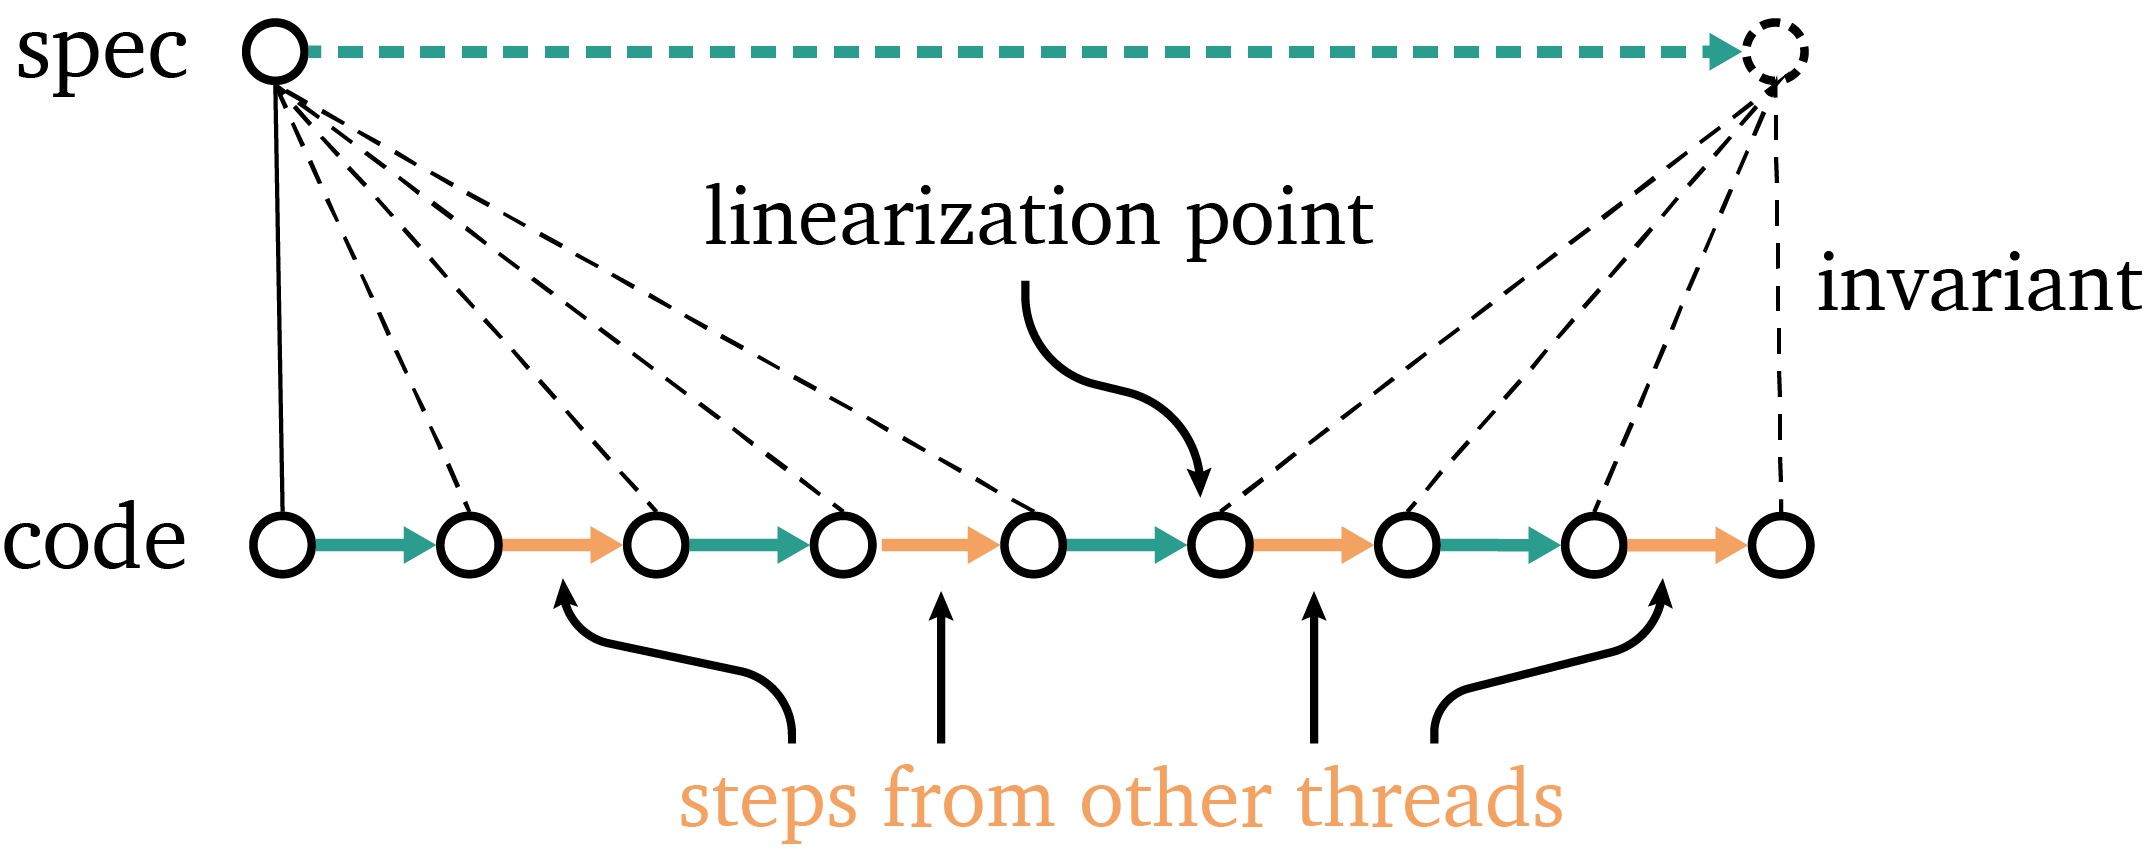
\includegraphics{fig/concurrent-refinement.png}
  \caption{Concurrent simulation}
  \label{fig:refinement:concurrent}
  \end{subfigure}%
%
  \begin{subfigure}[t]{0.4\textwidth}
  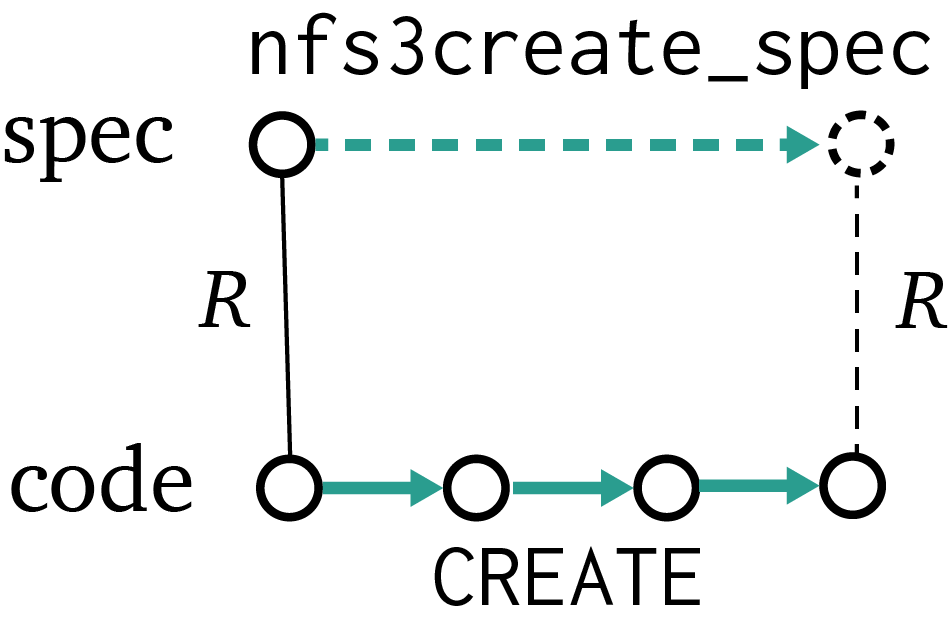
\includegraphics{fig/sequential-refinement.png}
  \caption{Sequential simulation}
  \label{fig:refinement:seq}
  \end{subfigure}
  \vspace{0.5\baselineskip}
  \caption[Proving a concurrent simulation]{Contrast between verifying a
    concurrent refinement (left) and sequential refinement (right), for a single
    procedure running the green-colored transitions. Proving concurrent
    refinement requires a proof that shows every operation (1) preserves the
    invariant at all intermediate points, and (2) simulates the abstract
    specification for the operation at some \emph{linearization point}. Unlike
    sequential refinement, the proof must show the invariant holds at
    intermediate points in order to reason about potential interference with
    other threads. \tej{fix vertical alignment}}

  \label{fig:concurrent-refinement}
\end{figure}


The design of DaisyNFS uses transactions, and in particular GoTxn, to simplify
the proof of concurrent refinement. Transactions appear to run
sequentially, and thus should permit reasoning about the body of each
transaction sequentially even though the actual execution interleaves multiple
transactions. This chapter describes a formalization of this intuition in the
form of a \emph{simulation-transfer theorem} (described in
\cref{sec:daisy:simulation-transfer}) which proves that a system implemented
with transactions that is verified with a sequential forward simulation against
some specification refines the same specification in the sense of a concurrent,
crash-safe refinement when run through GoTxn. The proof of this theorem is an
extension of the program refinement specification from \cref{sec:txn:spec}.

Due to simulation transfer, we are able to use a simpler verification
methodology of sequential simulation for the DaisyNFS file-system code, compared
to the Perennial program logic used to verify the transaction system underneath.
To fully take advantage of this difference, DaisyNFS is verified using
Dafny~\cite{leino:dafny}, an entirely different tool. Dafny is a
verification-oriented programming language that is restricted to sequential
proofs. The use of Dafny greatly reduces the proof burden for verifying
DaisyNFS, because sequential proofs are well-suited to automation and Dafny's
automation is well-developed (in contrast automation for concurrent proofs is
still nascent, and would need to be integrated into Perennial to be used for
these proofs).

The value of sequential proofs can be seen in the proof-to-code ratio for the
transaction system, which is $18\times$, versus the Dafny proofs which required
about $2\times$ as many lines of proof as code. Further evidence can be seen in
the incremental development of DaisyNFS, which \cref{sec:eval:incremental}
further elaborates on.

Simulation transfer greatly reduces the proof burden for verifying DaisyNFS.
There still remains a challenge of actually implementing the file system using
transactions. \Cref{sec:daisy:design} discusses some key challenges to address,
in particular how to ensure transactions are bounded in size (since GoTxn
transactions cannot exceed the size of the on-disk circular buffer) and avoiding
deadlocks in the transaction system.

The design of DaisyNFS does impose limitations. The proof approach relies on
transactions appearing to run sequentially, which prevents modifying state
outside the transaction system. This can be useful if verifying a system like a
persistent key-value store where some small metadata is manipulated with transactions, but
the bulk of the data is stored separately --- the proof of such a system would
require explicit crash and concurrency reasoning for the data reads and writes,
but GoTxn would still be useful for managing the metadata. GoTxn does not have a proof of liveness, and the file-system proof
does not show that transactions avoid deadlock. Our NFS implementation does not
cover some features, such as symbolic links, hard links, and paginated
\cc{READDIR}; we believe all of these could be implemented and specified with
the same approach but have not done so in our prototype.
